\section{Parallel reduction operations using OpenMP}
\subsection{Dot Product}
The implementation of the parallel versions of the Dot Product are given in Listing \ref{lst:red} and \ref{lst:crit}.
Important to note here is that the critical construct is not used to compute \texttt{alpha\_local} directly, which would lead to a serial code with an additional overhead. Rather compute the \texttt{alpha} locally on each thread and then use the critical construct to compute the final \texttt{alpha}. Both methods essentially perform a reduction operation, but is there a difference in performance? \newline
\begin{minipage}{.48\textwidth}
\begin{lstlisting}[language=C++, caption=Reduction Method, label=lst:red]
  for (int iterations = 0; iterations < NUM_ITERATIONS; iterations++) {
    alpha_parallel_red = 0.0;
#pragma omp parallel for reduction(+ : alpha_parallel_red)
    for (int i = 0; i < N; i++) {
      alpha_parallel_red += a[i] * b[i];
    }
  }

\end{lstlisting}
\end{minipage}\hfill
\begin{minipage}{.48\textwidth}
\begin{lstlisting}[language=C++, caption=Critical Section Method, label=lst:crit]
for (int iterations = 0; iterations < NUM_ITERATIONS; iterations++) {
	alpha_parallel_crit = 0.0;
	alpha_local = 0.0;
#pragma omp parallel firstprivate(alpha_local)
{
#pragma omp for
	for (int i = 0; i < N; i++) {
		alpha_local += a[i] * b[i];
	}
#pragma omp critical
	{
		alpha_parallel_crit += alpha_local;
	}
}
}

\end{lstlisting}
\end{minipage} \newline
In order to figure this out we use strong scaling analysis, where the amount of work stays constant (fixed size of the vector length) \cite{hager_introduction_2010}.
For this analysis we introduce a plot that compares the execution time per thread to the number of threads \ref{fig:scale}. Looking at the values of the plot, they appear to be identical,yet having a closer look at the actual values, we can see that the reduction method is a tiny bit faster, which is due to having a lower thread overhead compared to the critical implementation. For both methods we can clearly deduct that when increasing the number of threads from 1 to 16, we can see an significant decrease in execution time, while increasing the number of threads from 16 to 20 we either get a very small decrease in execution time or the execution even increases. This is mostly likely caused by the overhead caused the synchronization and the increased competition of resources, such as cache coherency and memory bandwidth.
Comparing the slope of the curves, in both cases we can clearly see that for vector sizes $10^5$ and $10^6$ the execution time decreases more rapidly, meaning when we add more threads to this vector size for small number of threads the speedup is a lot better and faster.
\begin{figure}[H]
    \centering
    \begin{subfigure}[b]{\textwidth}
        \centering
        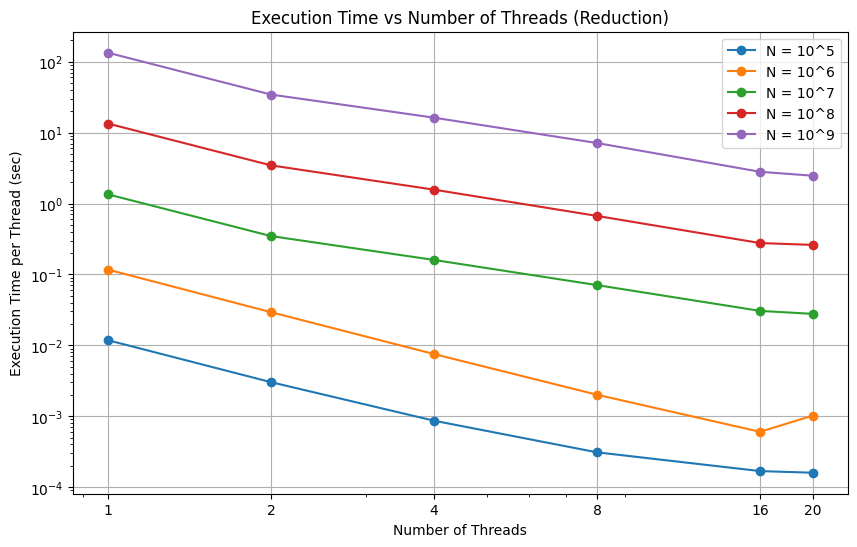
\includegraphics[width=\textwidth]{../media/execution_red.png}
        \caption{DotProduct using the Reduction clause}
        \label{fig:image1}
    \end{subfigure}
    \hfill \\
    \begin{subfigure}[b]{\textwidth}
        \centering
        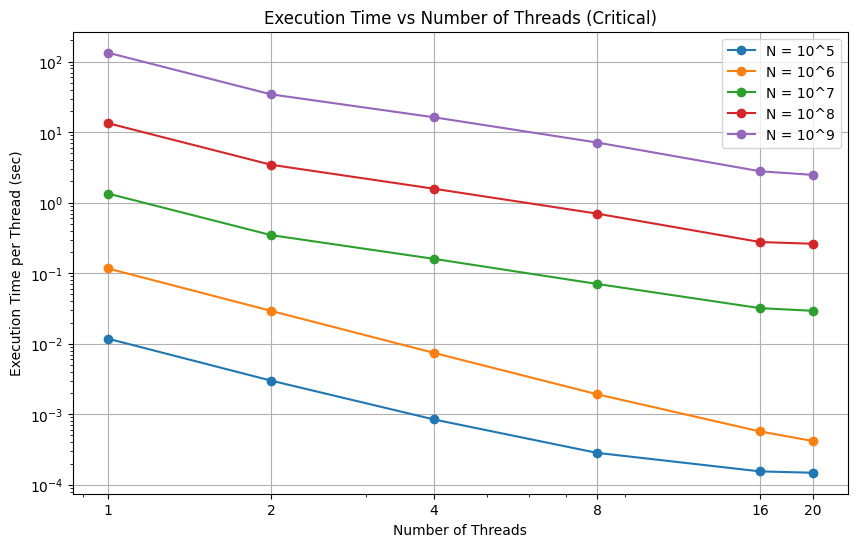
\includegraphics[width=\textwidth]{../media/execution_crit.png}
        \caption{DotProduct using the Critical section}
        \label{fig:image2}
    \end{subfigure}
    \caption{Strong scaling comparison of the Reduction method and the Critical Method using the execution time per thread}
    \label{fig:scale}
\end{figure}
 
\begin{figure}[H]
    \centering
    \begin{subfigure}[b]{\textwidth}
        \centering
        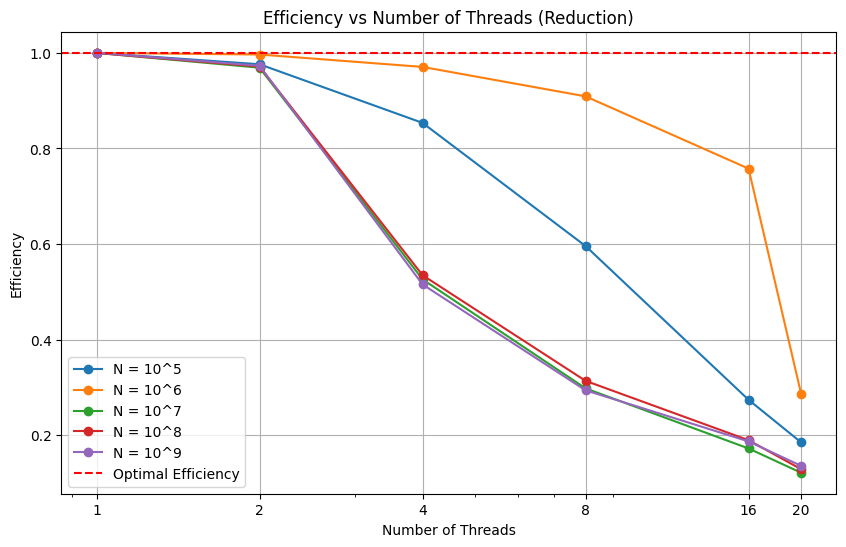
\includegraphics[width=\textwidth]{../media/eff_red.png}
        \caption{Efficiency of DotProduct using the Reduction clause}
        \label{fig:image1}
    \end{subfigure}
    \hfill \\
    \begin{subfigure}[b]{\textwidth}
        \centering
        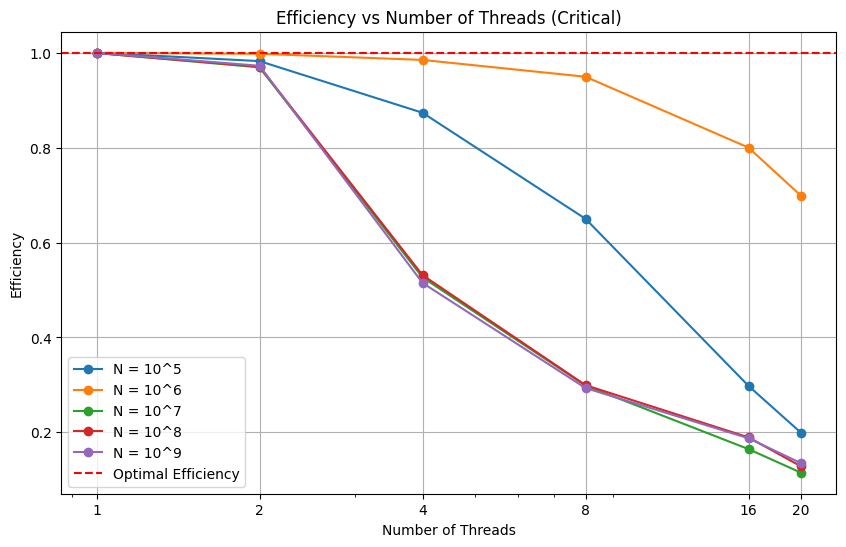
\includegraphics[width=\textwidth]{../media/eff_crit.png}
        \caption{Efficiency using the Critical section}
        \label{fig:image2}
    \end{subfigure}
    \caption{Efficiency comparison of the Reduction method and the Critical Method}
    \label{fig:eff}
\end{figure}
\newpage
Another question posed in scalability is how effectively can a given resource be used in a parallel program \cite{hager_introduction_2010}. We can define parallel efficiency as 
\begin{equation} \label{eq:eff}
E = \frac{T_1}{n T_n}
\end{equation}
where $T_n$ is the execution time of thread n-th thread.
Looking at the efficiency plots in Figure \ref{fig:eff}, we can observe once more that both methods critical and reduction behave almost identical.
The plot also clearly shows that for vector sizes $10^5$ and $10^6$ can use the small number of threads more efficiently, while for a higher number of threads they experience a sharp drop in efficiency. This suggests that for higher number of threads the managing of threads is high in comparison to the computational work. For a larger vector size initially there's a large decline of efficiency, but with increasing number of threads the decline is rather gradual, which makes sense, since large arrays can distribute their elements more effectively over a large number of threads. In addition for a larger array, the time OpenMP needs to create and manage threads is lower in relation to the time the threads needs to compute the dot product. If we compare the different vector sizes with the optimal efficiency then the for the two smallest vector sizes are the most efficient or in other words closest to the optimal efficiency.\newline
\newline
At what point the multi-threaded version of the dot product becomes beneficial depends on the balancing of the overhead versus the amount of work per thread. This is usually indicated by a sharp drop in the efficiency plot. In our case beneficial for all $N$ because the multi-threaded version is faster than the serial, but it is important not to use too many threads, depending on the vector size.    
\subsection{Approximating $\pi$}
For my parallel version of pi simply use \texttt{omp parallel for} directive to distribute the work over the available threads. In addition I use the reduction clause to ensure the safe combination of the individual sums coming from each thread, avoiding race conditions when multiple threads write to a shared variable. The load balancing is done automatically by OpenMP, which should be well optimized for such a simple operation. 
\begin{lstlisting}[language=C++, caption=Serial and Parallel implementation of Pi, label=lst:pi]
  /*  Serial Version of Computing Pi*/
  for (long long int i = 0; i < N; i++) {
    x = dx * (i + 0.5);
    sum += 4 / (1 + x * x);
  }
  pi = sum * dx;

  /*  Parallel Version of Computing Pi*/
  sum = 0.;
#pragma omp parallel for reduction(+ : sum)
  for (long long int i = 0; i < N; i++) {
    x = dx * (i + 0.5);
    sum += 4 / (1 + x * x);
  }
  pi = sum * dx;
\end{lstlisting}
The speedup is defined by the ratio
\begin{equation}
	S_n = \frac{T_1}{T_n}
\end{equation}
where $T_1$ and $T_n$ are the execution time of the serial and parallel version with $n$ threads.
It shows us how much faster a parallelized program runs in comparison to its serial counterpart.
The optimal (theoretical) speedup is only achievable with perfect parallelization, where no overhead or bottlenecks exist and is proportion to the number of threads $S_n = n$. In realty this not achievable, because in order to run a program in parallel we always have an overhead for communication, synchronization, load balancing among others.
There are different types of speedup plots we can look at in this case we look at strong scaling problem, which means the input size stays fixed at vector length $10^{10}$. \newline
The efficiency is closely related to the speedup and as seen in equation \ref{eq:eff}, it is the speedup divided by the number of threads.\newline
\newline
Looking at the results of the speedup plot in Figure \ref{fig:pi_speedup}, this implementation of computing Pi comes very close to the optimal speedup, which means that the overhead is being held to a minimum and adding an additional thread halves the execution time. In terms of efficiency for this program it is very close to 1 and creates approximately a constant line. 
\begin{figure}[H]
    \centering
        \centering
        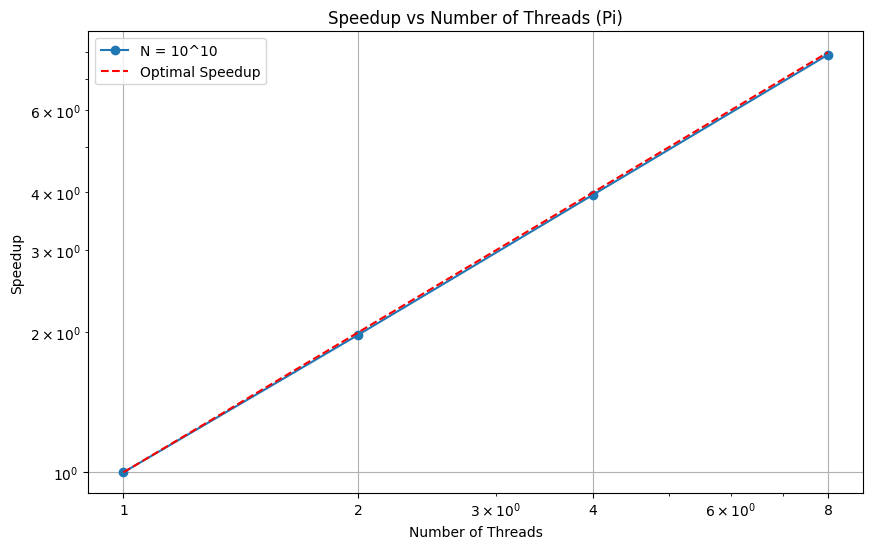
\includegraphics[width=\textwidth]{../media/pi_speedup.png}
        \caption{Speedup plot for computing pi}
        \label{fig:pi_speedup}
    \end{figure}

